\section{Introducción}
\subsection{Persistencia de visión}
La persistencia de visión (\textsl{Persistence Of Vision}/\textbf{POV} en
Inglés) es un fenómeno óptico por el cual las imágenes que percibimos permanecen
aproximadamente durante $\frac{1}{25}s$. Esto hace posible que percibamos
movimiento como continuo, en lugar de como una sucesión de imágenes estáticas.

\begin{figure}[!ht]
	\centering
	\begin{subfigure}[t]{0.4\textwidth}
		\centering
		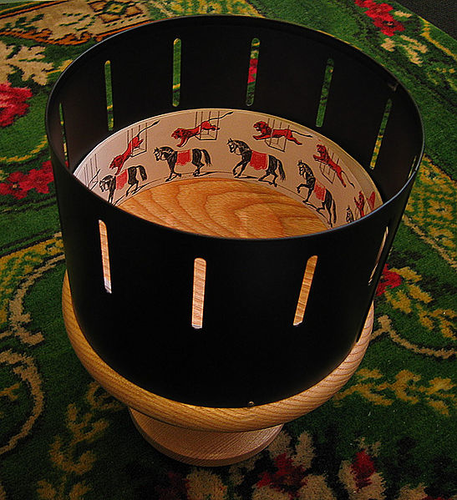
\includegraphics[width=\textwidth]{images/Zootropo}
		\caption{Zoótropo}
	\end{subfigure}
	\hspace{0.5cm}
	\begin{subfigure}[t]{0.4\textwidth}
		\centering
		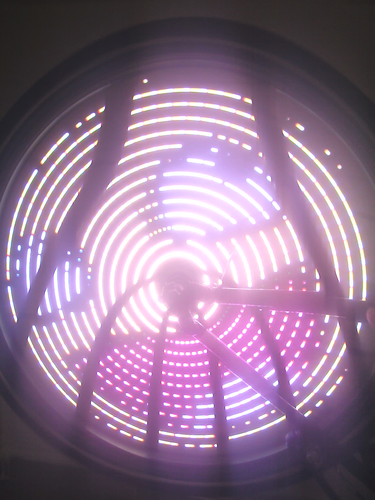
\includegraphics[width=\textwidth]{images/awesomeByke}
		\caption{CyclePOV}
	\end{subfigure}
	\caption{Ejemplos de aplicaciones que aprovechan el POV}
\end{figure}

\subsection{Objetivos}
El objetivo principal del proyecto es conseguir un efecto de persistencia de
visión en la rueda de una bici, de forma que se puedan apreciar imágenes y
animaciones con el movimiento de la misma. Para ello utilizamos tiras de LEDs
RGB direccionables unidas a los radios de la rueda, y controladas con una placa
\textsl{STM32F4-Discovery} utilizando \uCOS .

También implementamos una comunicación mediante infrarrojos para poder
comunicarnos con el sistema mientras está girando, con la intención de enviarle
comandos e imágenes.

\subsection{Estado del arte}
Existen multitud de sistemas como el que estamos construyendo y otros tantos
parecidos que también se aprovechan de la persistencia de visión.

Hay empresas como \textbf{MonkeyLectric} (\url{http://www.monkeylectric.com})
que comercializan productos como el que hemos construido
(\reffig{fig:monkeyLight}).

Otros sitemas parecidos utilizan un motor para hacer girar los LEDs formando
un plano circular (\reffig{fig:clock}), un cilindro (\reffig{fig:cylinder}) o
una esfera (\reffig{fig:sphere}).

Por último, también hay sistemas en los que el movimiento de los LEDs se realiza
con la mano. Se valen de una IMU (\textsl{Inertial Measurement Unit} - Unidad de
medición inercial) para calcular la velocidad del movimiento y cambiar los LEDs
en el momento adecuado (\reffig{fig:handPOV}).

\begin{figure}[!p]
	\centering
	\begin{subfigure}[t]{0.3\textwidth}
		\centering
		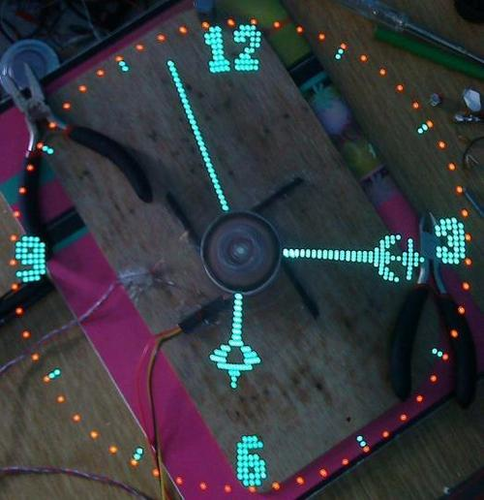
\includegraphics[width=\textwidth]{images/clock}
		\caption{Reloj. LEDs girando en plano circular.}
		\label{fig:clock}
	\end{subfigure}
	\hspace{0.5cm}
	\begin{subfigure}[t]{0.3\textwidth}
		\centering
		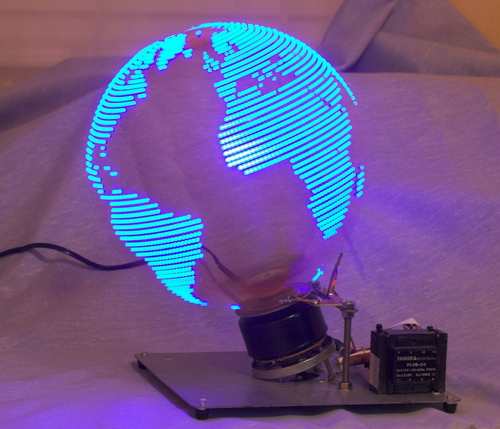
\includegraphics[width=\textwidth]{images/sphere}
		\caption{Esfera. Arco de LEDs girando sobre un eje central.}
		\label{fig:sphere}
	\end{subfigure}
	\\
	\begin{subfigure}[t]{0.3\textwidth}
		\centering
		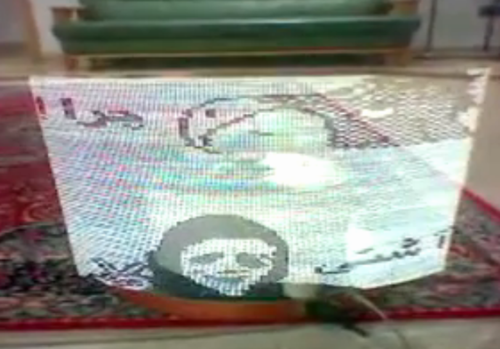
\includegraphics[width=\textwidth]{images/cylinder}
		\caption{Cilindro. Linea de LEDs girando sobre un eje central.}
		\label{fig:cylinder}
	\end{subfigure}
	\hspace{0.5cm}
	\begin{subfigure}[t]{0.3\textwidth}
		\centering
		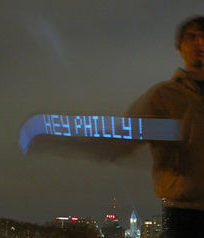
\includegraphics[width=\textwidth]{images/handPOV}
		\caption{Móvil utilizando su IMU para dibujar texto con el
		movimiento de la mano.}
		\label{fig:handPOV}
	\end{subfigure}
	\\
	\begin{subfigure}[t]{0.4\textwidth}
		\centering
		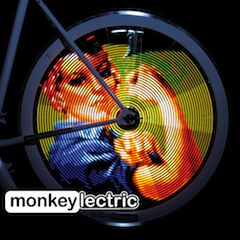
\includegraphics[width=\textwidth]{images/monkeyLight}
		\caption{Producto de la empresa MonkeyLectric}
		\label{fig:monkeyLight}
	\end{subfigure}

	\caption{Diversos sistemas que utilizan la POV con LEDs en movimiento.}
\end{figure}
